\section{Evaluation}\label{sec_evaluation}
In this section, we evaluate the proposed approach using  synthesized automotive applications that conform  to the automotive benchmark proposed by Kramel et al.~\cite{Kramer2015RealFree}. The number of runnables, timing specification and activation patterns within the cause-effect chains are also selected according to the benchmark. In order to show the scalability of our approach and to assess the scope of its applicability in practice, in some cases, we use higher specifications standard  than what is indicated in the benchmark, e.g., the maximum number of activation patterns is extended from three to four.

In the rest of the section, we describe the setup and method of evaluation, followed by discussion of the evaluation results.

%\subsection{Preparation}
\subsection{Setup}
The evaluation setup consists of three hardware platforms with different computing capacities, i.e., processing speed and memory size as shown in Table~\ref{tbl_hardwaremodel}. The evaluation on different platforms can be used as performance indicator and also to identify performance bottlenecks in the model. HP EliteBook and Lenovo 20378 are personal computers with core-i5 and core-i7 processors, respectively, whereas PowerEdge is a workstation with much higher processing and memory specification than the personal computers.
\begin{table}[h]
\centering\small
\begin{tabular}{@{}p{0.25\columnwidth}p{0.275\columnwidth}llll@{}}
\toprule
Hardware Model  & Pro. Model & \rotatebox{70}{\#Pro.} & \rotatebox{70}{\#Core} & \rotatebox{70}{Cache} & \rotatebox{70}{RAM}\\ \midrule
$^1$HP EliteBook & $^3$Core i5, 2.2GHz & 1 & 2 & 3M & 8G \\ 
Lenovo 20378 & $^4$Core i7, 2.6GHz & 1 & 4 & 6M & 16G\\ 
$^2$PowerEdge & $^5$Xeon(R), 2.4GHz & 24 & 6 & 15M & 256G\\
\bottomrule
\end{tabular}
\caption{Summary of the Hardware Specifications.\\
\footnotesize{$^1$HP EliteBook 840 G2, $^2$PowerEdge R730 Rack Server}\\
\footnotesize{$^3$Intel® Core™ i7-4720HQ @ 2.60GHz, $^4$Intel® Core™ i7-4720HQ @ 2.60GHz $^5$Intel(R) Xeon(R) CPU E5-2620 v3 @ 2.40GHz}}
\label{tbl_hardwaremodel}
\end{table}

\subsubsection{Software Application Benchmark} In order to evaluate the proposed approach on different ranges of applications, we automatically generate synthetic examples that comply with the automotive benchmark~\cite{Kramer2015RealFree}. The examples denote simple to complex automotive functions such as reverse-parking assistance system and engine control system. For simplicity, we identify three classes of applications with different sizes and complexity, shown as tuple $(c, r, t, g)$, respectively for the number of software components, runnables, tasks, and cause-effect chains. Table \ref{tbl_appsspec} shows the range of values used in the applications for evaluation. 
\begin{table}[h]
\centering\small
\begin{tabular}{@{}llll@{}}
\toprule
Parameter  		& Spec.-I  & spec.-II & spec.-III\\ 
\midrule
components, $c$		& $\leq 10$	& $\leq 15$ 	& $> 15$\\ 
runnables, $r$		& $\leq 50$	& $\leq 100$ 	& $> 100$\\
tasks, $t$ 			& $\leq 30$ & $\leq 60$ 	& $> 60$\\
cause-effect chains, $g$ & $\leq$ 30 & $\leq$ 40 & $> 60$\\ \midrule
activation-pattern	& \multicolumn{3}{c}{$[2,3,4]$}\\ \midrule
share of activation-patterns	& \multicolumn{3}{c}{$[0.7, 0.2, 0.1]$}\\
\bottomrule
\end{tabular}
\caption{Specification of the Applications for Evaluation.}
\label{tbl_appsspec}
\end{table}

\subsubsection{Platform Benchmark} The specification of nodes can be obtained from simulation, vendor product specification and  experience. Figure~\ref{tbl_nodesspecs} shows the range of values that are used in the nodes' specification. In the experiment, the values are randomly generated while respecting the benchmark.
\begin{table}[h]
\centering\small
\begin{tabular}{@{}llll@{}}
\toprule
Parameter  		& Range\\ 
\midrule
nodes							& $4-10$\\
power consumption (Watt), $p$ 	& $10 - 200$\\
failure-rate (/Mhr), $\lambda$ 	& $10^4 - 10^{-2}$\\
speed factor, $hz$			 	& $0.0 - 1.0$\\
\bottomrule
\end{tabular}
\caption{Range of Values for the Specification of Nodes.}
\label{tbl_nodesspecs}
\end{table}

\subsection{Result}
We conduct three experiments that assess the proposed approach for scalability in terms of \textit{allocation time}. The allocation time is defined as the time required to prepare and solve the allocation problem using the proposed ILP method. Furthermore, we show resource efficiency in terms of saving nodes (i.e., using smaller number of nodes). The experiments consist of: i) varying the size of applications in order to observe the effect of increasing components, runnables and tasks in the system, ii) varying the complexity of applications in order to observe the effect of cause-effect chains in the system, and iii) varying the replications. The experiments are discussed in detail in the next subsection.

A preliminary analysis of the evaluation indicates a successful termination of the allocation for Spec-I\&II of the applications. Whereas for Spec-III, the allocation problem is intractable. In fact, it took days on the PowerEdge machine and many times it did not terminate successfully. Therefore, the experimental results that are shown in this paper are conducted on the Spec-I\&II classes. 
\begin{figure*}
    \centering
    \begin{subfigure}[b]{0.525  \textwidth}
        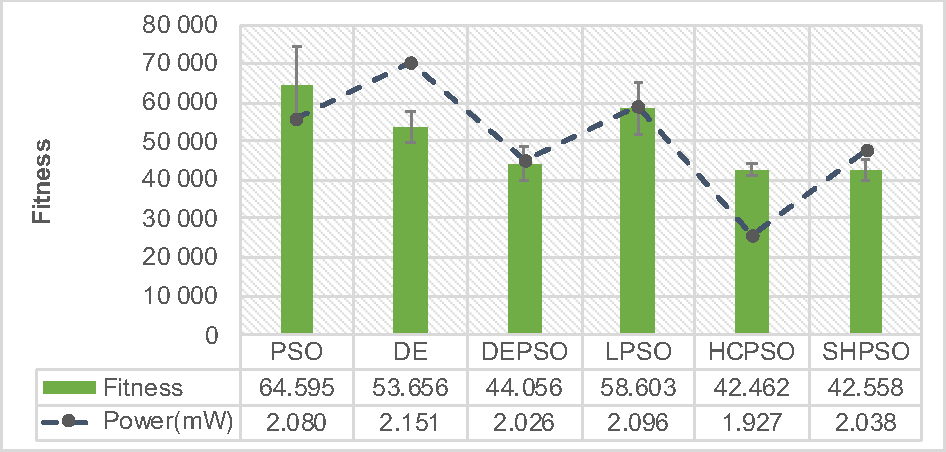
\includegraphics[width=\textwidth]{img/fitness_c20_g30_m10.pdf}
        \caption{Fitness and Power Consumption.}
        \label{fig_util}
    \end{subfigure}
    ~%\hspace{-0.4cm}
        \begin{subfigure}[b]{0.45\textwidth}
        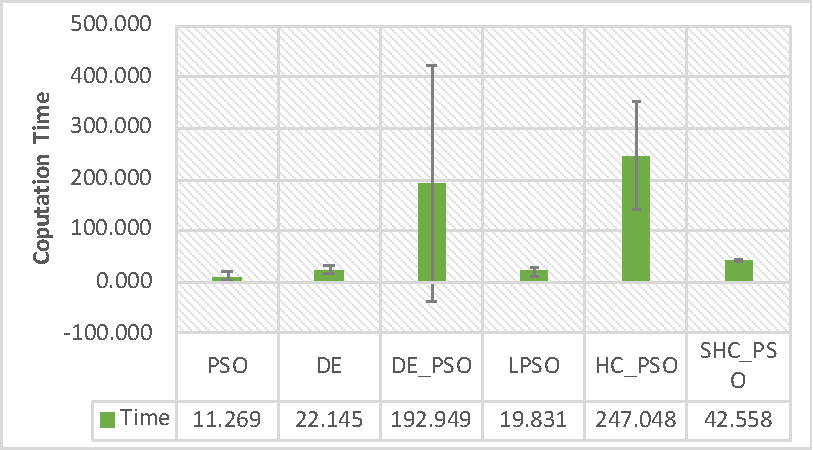
\includegraphics[width=\textwidth]{img/time_c20_g30_m10.pdf}
        \caption{Computation Time}
        \label{fig_power}
    \end{subfigure}
    \caption{Allocation of Software Application $(N_c=20,N_r=200,N_\Gamma=30)$ on $N_m$ number of Heterogeneous Nodes using Different Optimization Methods.}
    \label{fig_util_power}\vspace{-0.2cm}
\end{figure*}



\begin{figure}[t!]
\centering
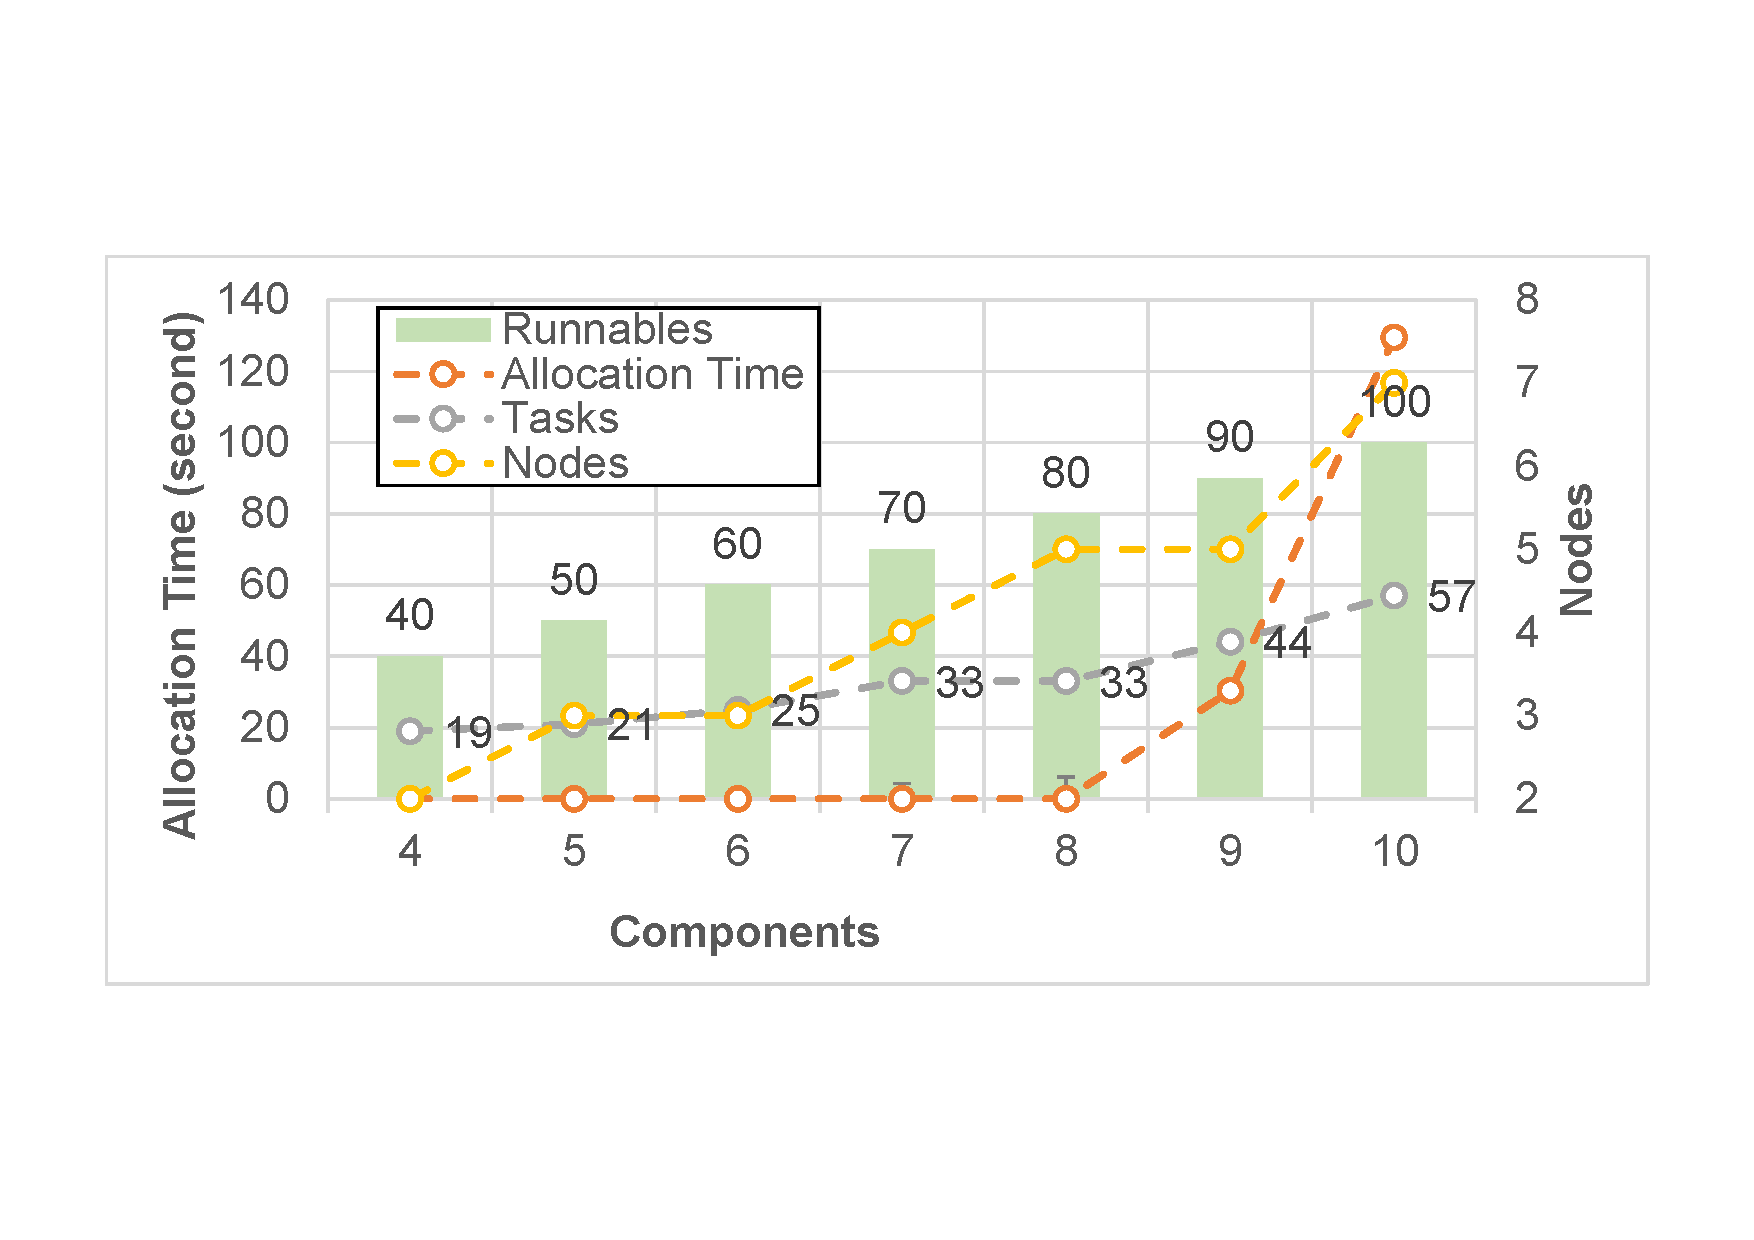
\includegraphics[width=0.7\linewidth]{increasing_components}
\caption{Effect of Varying the Application Size on the Allocation Time and Number of Utilized Nodes.}
\label{fig_increasing_components}
\end{figure}

\subsubsection{ILP Evaluation}
\paragraph{Varying the Size of Application} 
This refers to increasing the number of software components, as well as runnables, tasks, and cause-effect chains in the system. Figure~\ref{fig_increasing_components} shows the effect of increasing the size of an application from $(c4,r40,t19,g30)$ to $(c10,r100,t57,g60)$ on the allocation time and  the number of nodes utilized. The applications are allocated to a pool of 8 heterogeneous nodes sharing a single network and with specifications shown in Table~\ref{tbl_nodesspecs_exp}. The specifications are generated randomly, with uniform distribution, within the scope of Table~\ref{tbl_nodesspecs}.
% Please add the following required packages to your document preamble:
% \usepackage{booktabs}
\begin{table}[]
\small
\begin{tabular}{@{}llllllll@{}}
\toprule
Application & Measure & PSO & LPSO & DE & DEPSO & HCPSO & SHPSO \\ \midrule
App1 & Mean &  &  &  &  &  &  \\
 & Std.Dev. &  &  &  &  &  &  \\
App2 &  &  &  &  &  &  &  \\ \bottomrule
\end{tabular}
\end{table}

\begin{figure*}
    \centering
    \begin{subfigure}[b]{0.4  \textwidth}
        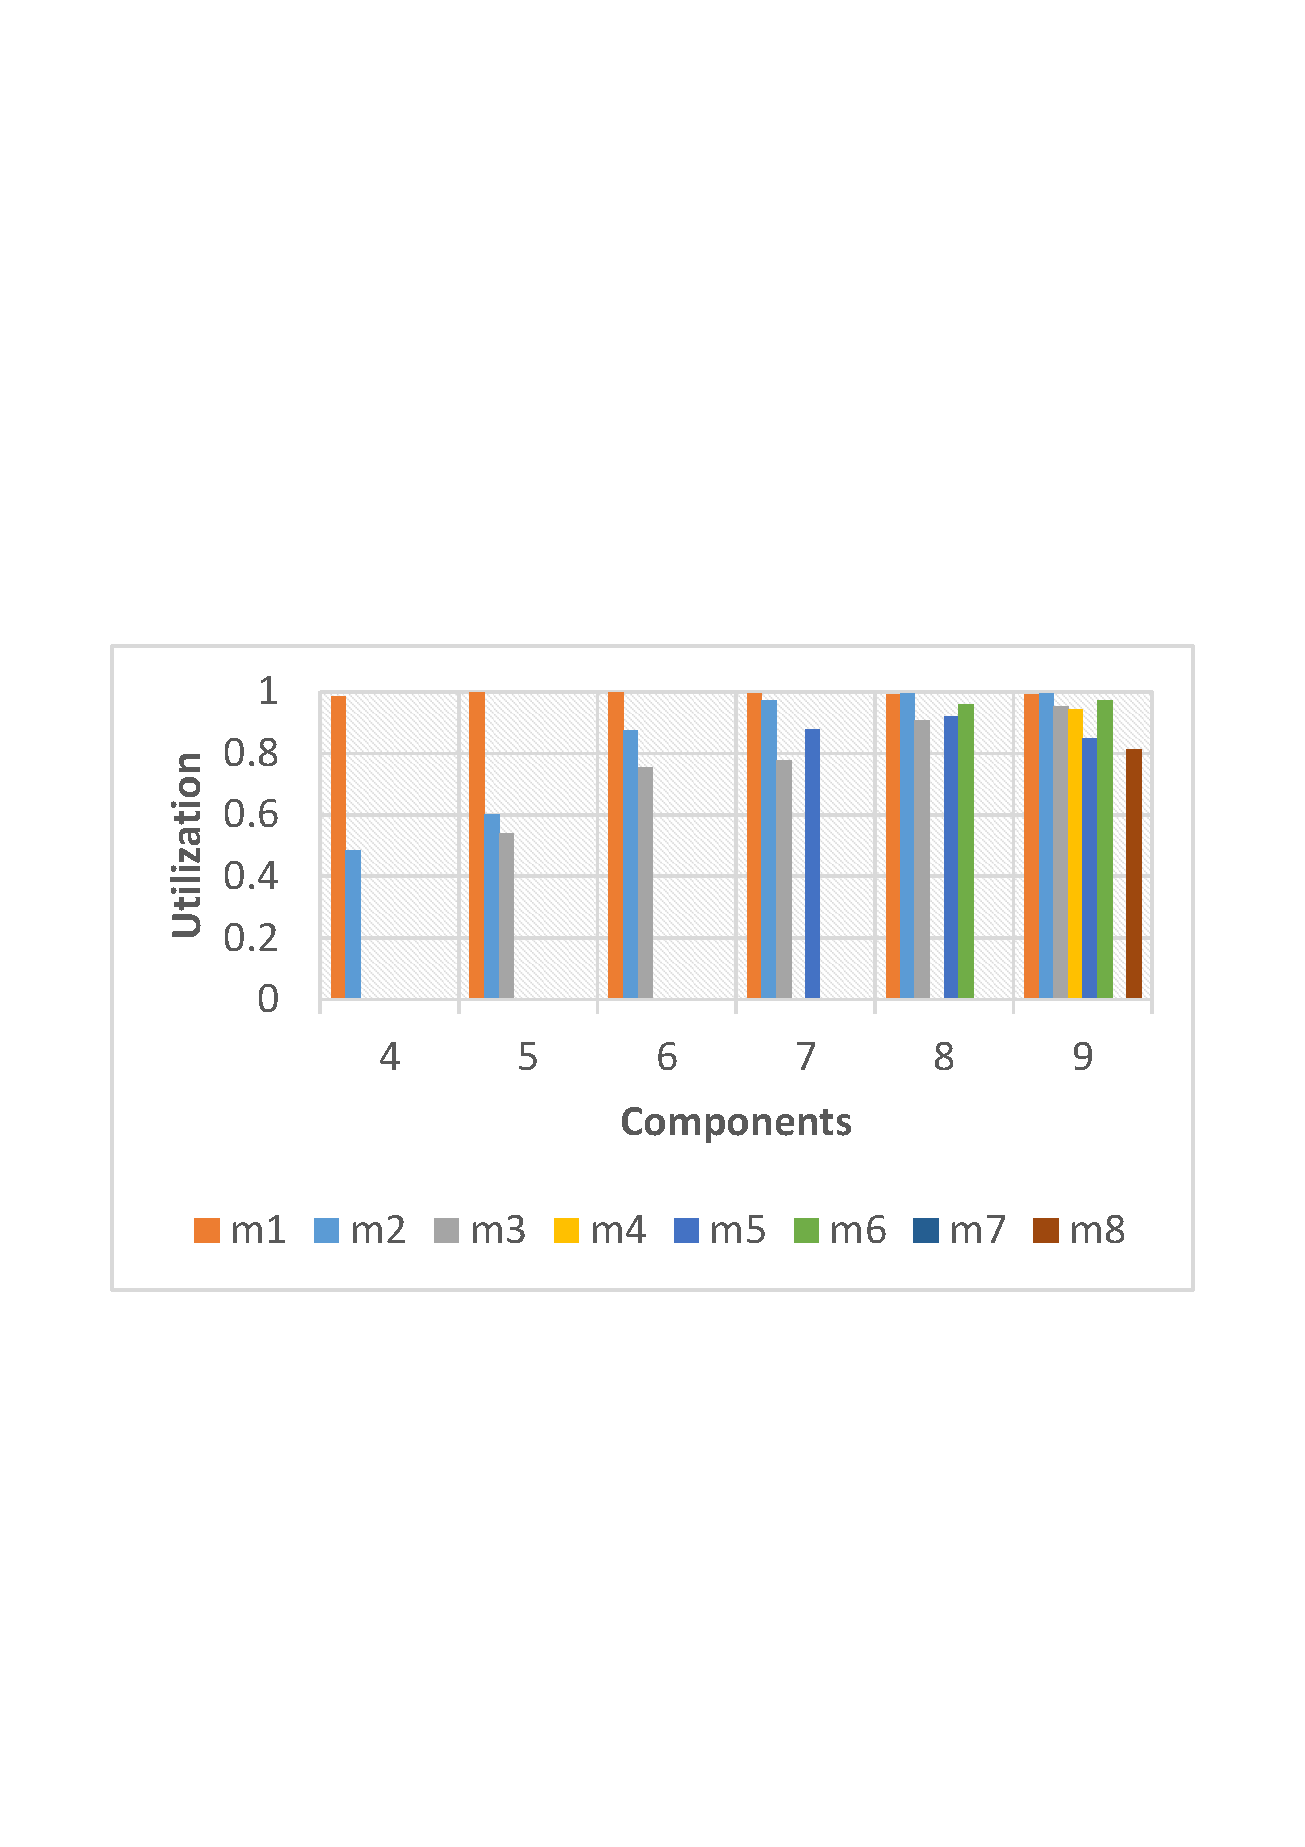
\includegraphics[width=\textwidth]{util}
        \caption{Utilization of Nodes.}
        \label{fig_util}
    \end{subfigure}
    ~%\hspace{-0.4cm}
        \begin{subfigure}[b]{0.4\textwidth}
        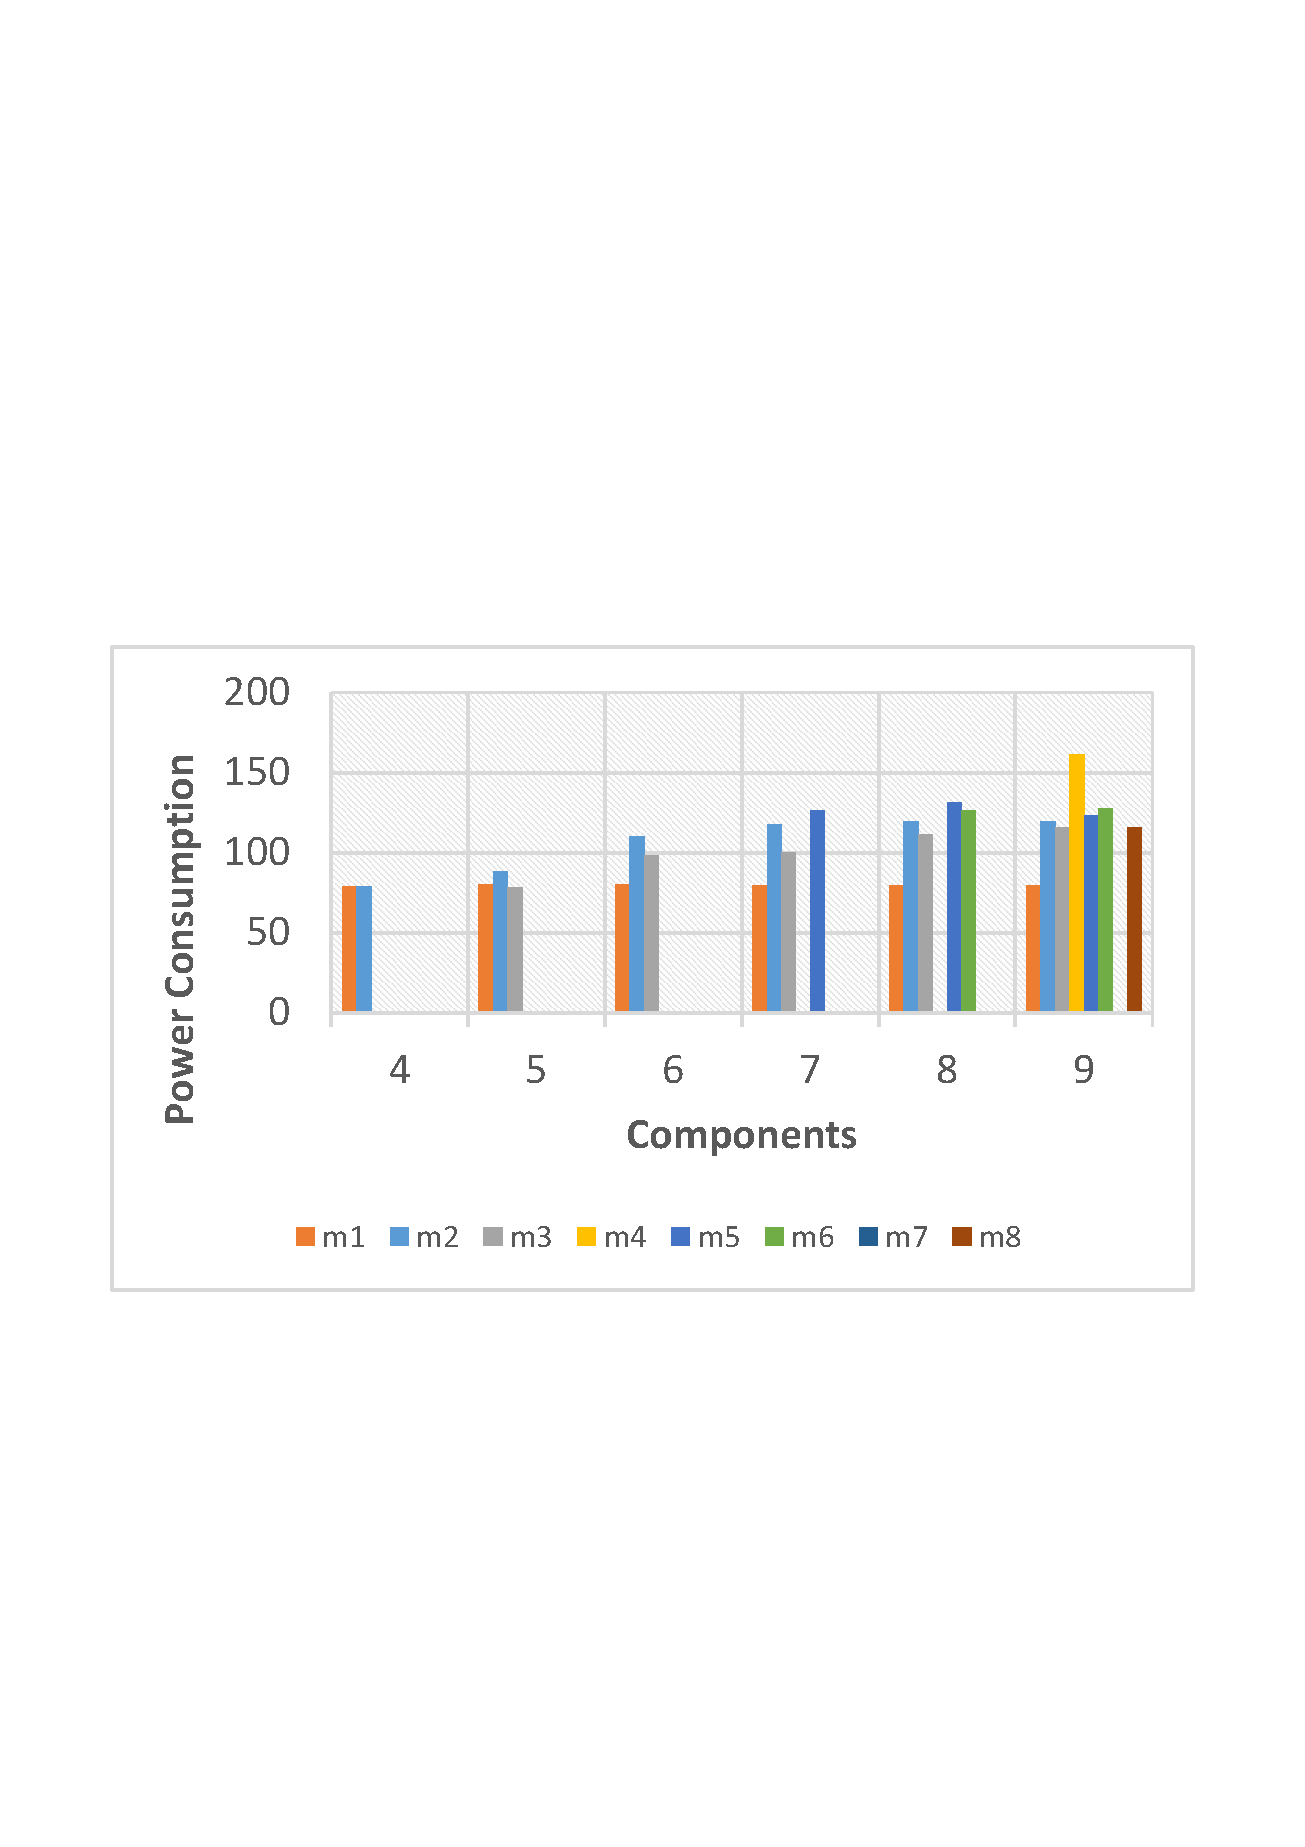
\includegraphics[width=\textwidth]{power}
        \caption{Power Consumption of Nodes.}
        \label{fig_power}
    \end{subfigure}
    \caption{Allocation of Applications on Heterogeneous Nodes.}
    \label{fig_util_power}\vspace{-0.2cm}
\end{figure*}

The CPLEX solver returns an optimal solution for the application $(c8, r80,t44,g30)$ within 6.06 sec. The allocation time increased sharply to 30.3 sec and 129.4 sec respectively for 9 and 10 components. Even if not indicated in this chart, the solver, the solver returns an optimal solution within 45 min for components reaching 15 on the PowerEdge machine and OutOfMemory error on the Lenovo and HP machines. Figure~\ref{fig_util} and Figure~\ref{fig_power} show the utilization and power consumption on each node for the different application sizes. The optimal allocation, in the general case, favor nodes with higher processor speed and lower power consumption specifications.

\paragraph{Varying the Number of Cause-effect Chains} 
In order to observe the effect of increasing the cause-effect chains on the allocation time, we vary the number of chains in the application from 10 to 60, which is consistent with the benchmark~\cite{Kramer2015RealFree}. The share of activation patterns also increases proportionally with the ratio $1:[0.7, 0.2, 0.1]$, respectively, for two, three, and four activation patterns. For instance, out of 10 cause-effect chains, there are 7 chains (with two activation patterns), 3 chains (with three activation patterns), and 1 chain (with four activation patterns). The experiment is conducted on two cases of schedulability analysis, namely response time analysis (RTA) and utilization bound (UB), and their result is shown in  Figure~\ref{chart_cause_effect_chain} for increasing number of chains.
\begin{figure}[h!]
\centering
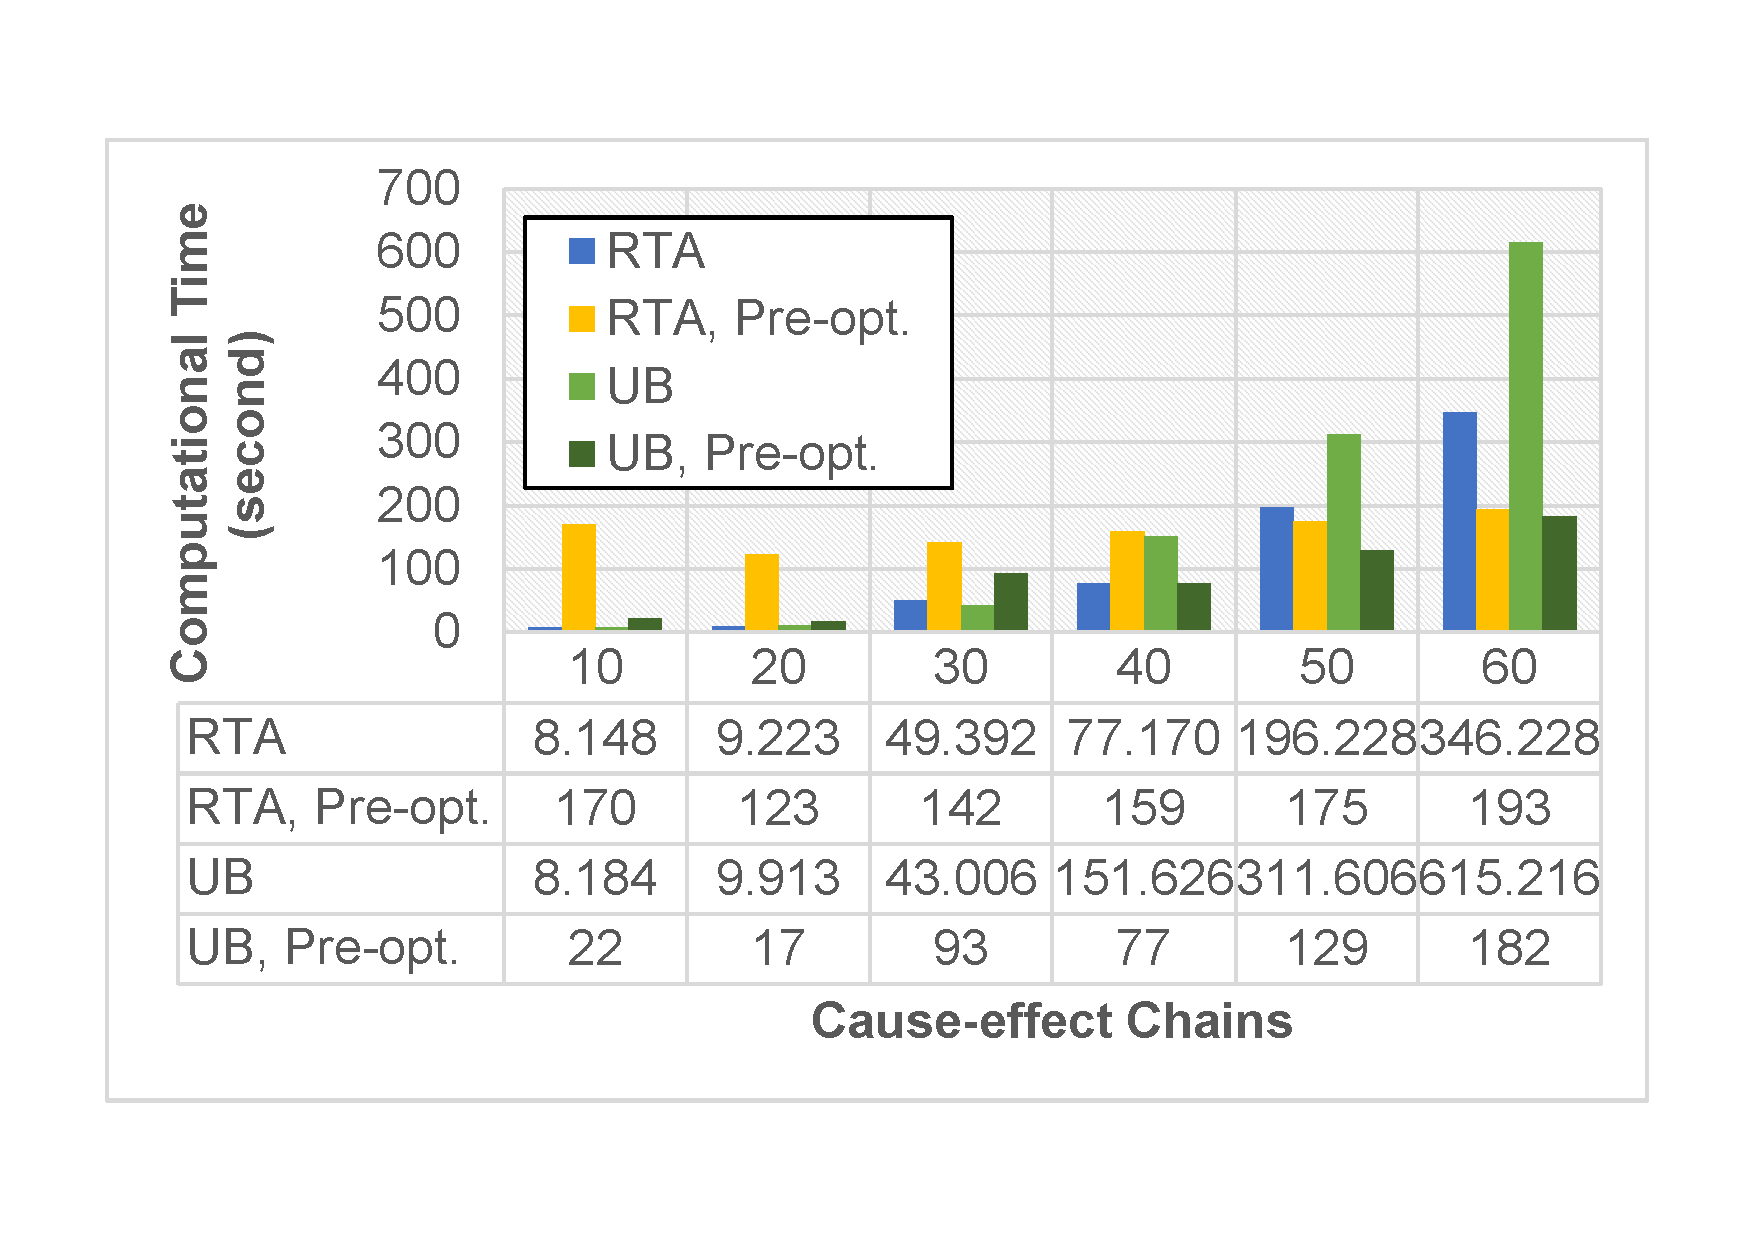
\includegraphics[width=0.7\linewidth]{increasing_cause-effect_chains}
\caption{Effect of Increasing Cause-effect Chains (under RTA and UB) on the Allocation Time.}
\label{chart_cause_effect_chain}\vspace{-0.4cm}
\end{figure}

The figures in the data table show an exponential growth of allocation time whenever the cause-effect chains are increased linearly for a specific application, in both cases of schedulability analysis. In the case of RTA, the overhead in the pre-optimization is higher than the overhead in the optimization for 50 or less chains. Whereas in the UB case, the computational time of pre-optimization is almost always less than the computational time of the optimization. 
The results are consistent with our expectation that the RTA computation, in the preparation of the timing assertions, is expensive, albeit provides schedulable tasks allocation based on the fixed-priority scheduling policy. In contrast, the UB computation time is relatively low; however, the search space gets larger due to more and more feasible tasks partitioning and chains fulfilling the timing constraints. As a result, the optimization time in the case of UB is usually higher as compared to the case of RTA. Therefore, for applications with chains not more than 40 and naive scheduling assumption using UB, the experiments favor the UB assumption. Whereas, the allocation with the RTA assumption should be selected for applications with exact scheduling requirements. Note, the scalability of this experiment should be seen in conjunction with the experiment discussed in the previous subsection.

\paragraph{Varying Replications}
In this experiment, we evaluate the allocation time of the applications with the increase in the number of replications. For the applications specification shown in Figure \ref{fig_replication}, we vary the replications from 1 to 4. 
The allocation in all applications took not more than 10 sec for replications 1 and 2. For Spec-I with replication 3 and 4, the allocation time went up close to 1 min. For Spec-III with replication 3, the allocation time went up rapidly to 30 min, and took extremely large time for replication 4 which is also the case for Application-II.
\begin{figure*}[h]
    \centering
    \begin{subfigure}[b]{0.475\textwidth}
        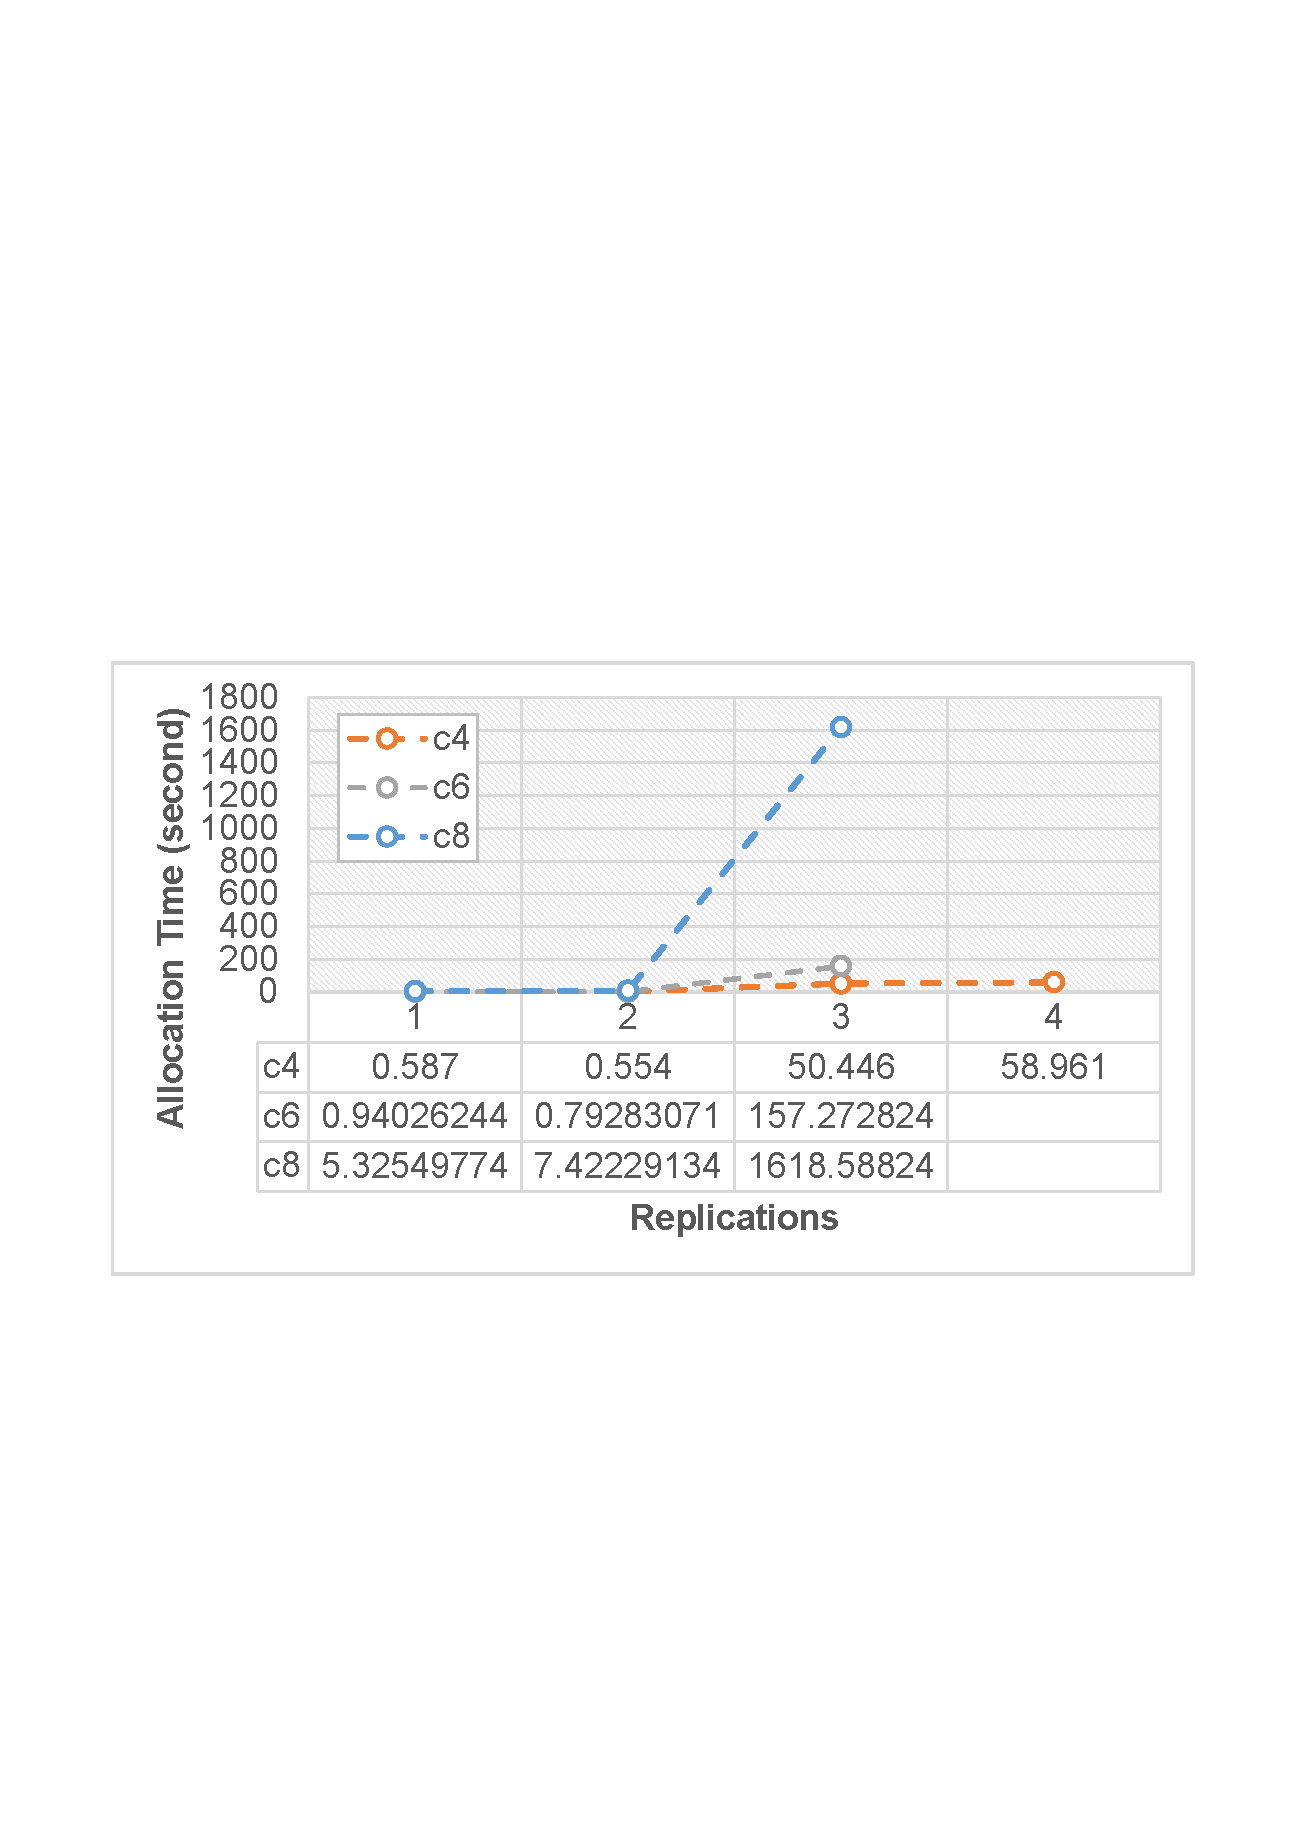
\includegraphics[width=\textwidth]{replications}
        \caption{Effect on Allocation Time.}
        \label{fig_replication_1}
    \end{subfigure}
    ~
        \begin{subfigure}[b]{0.475\textwidth}
        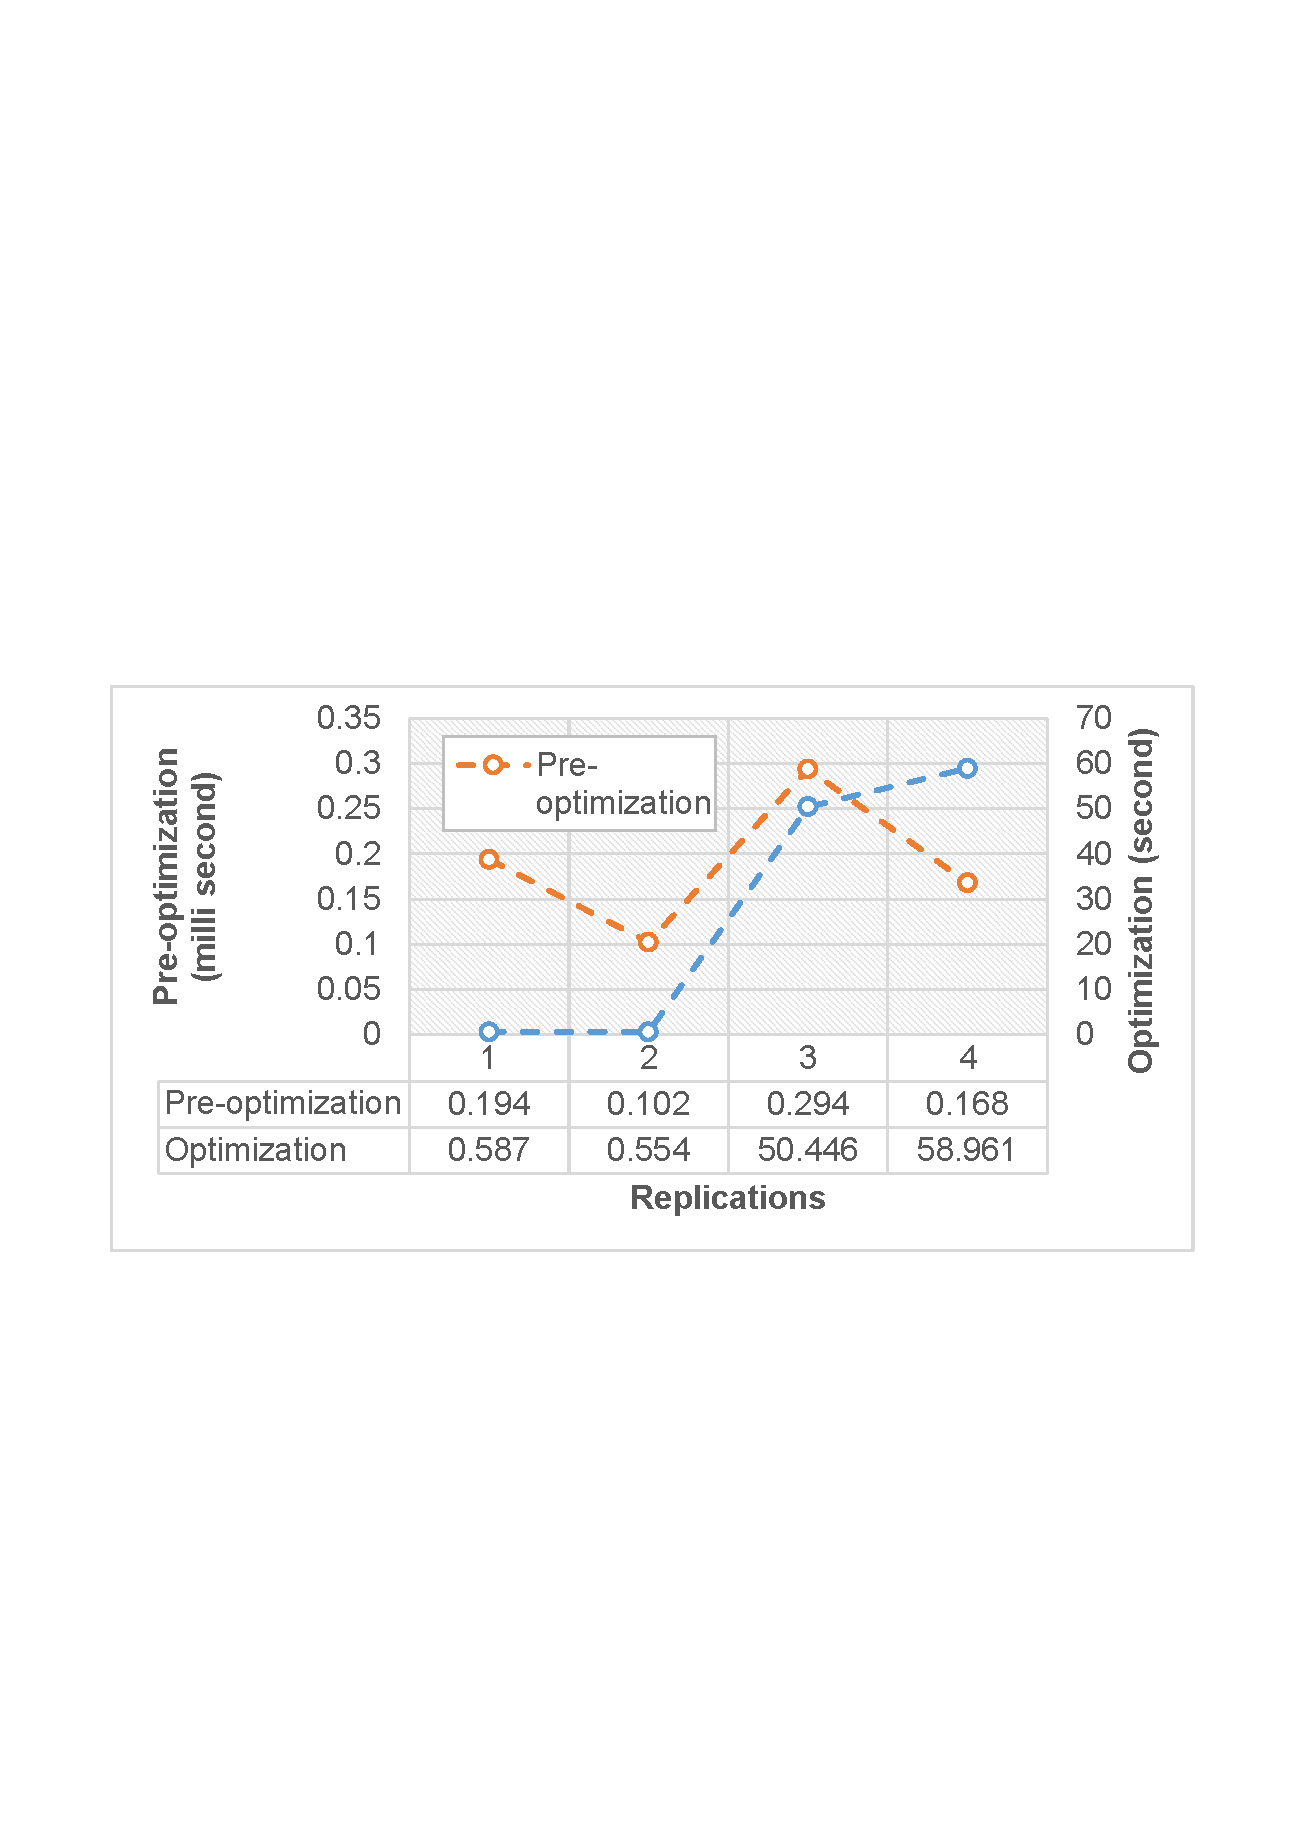
\includegraphics[width=\textwidth]{replication_comparison}
        \caption{Effect on Pre-optimization.}
        \label{fig_replication_2}
    \end{subfigure}
    \caption{Effect of Varying the Component Replications on the Allocation Time.}
    \label{fig_replication}\vspace{-0.5cm}
\end{figure*}

Figure~\ref{fig_replication_2} shows the effect of shared constraints on the overhead of replications during the pre-optimization and optimization phases of the allocation. In the pre-optimization phase, the allocation time was stable for the increased size of applications. This is due to the fixed constraints regardless of the replications. In contrast, the allocation time increases during optimization as the constraints are applied for the various combination of task partitions, cause-effect chains, and reliability states generated as the result of replications.

\subsection{Metaheuristic Evaluation}
Clearly, the ILP evaluation shows that the ILP approach does not scale to large software allocation problems, that is, that allocation time increases exponentially as the size of the software application increases. In fact, the allocation does not return results for applications consisting more than 15 software components. In this subsection, we evaluate ILP in conjunction with the PSO, DE, and hybrid PSO techniques for different problem sizes.

Table \ref{tbl_fitness_allocationtime_ilp_plus_metaheuristic} shows the fitness values and allocation time of the different algorithms for the increasing sizes of the software allocation problems. For no constraints violations, the fitness values denote the total power consumption, which is the case for the first three problems whereas it is not the case for the last three problems, thus the fitness values extremely increased as more violations are made. Furthermore, the algorithms highlighted in bold shows the benchmark for the corresponding specific problems. 

The result shows that the ILP approach returned solutions for the first three problems, in which case it becomes the benchmark for the quality assessment of the metaheuristic algorithms. Whereas, for the last three problems, ILP does not return solution, which conforms the previous ILP evaluation results. The metaheuristic results are further discussed as follows, that is with regard to solution quality and computation time.

\paragraph{Solution Quality} For the first problem, which models the smallest software allocation over heterogeneous nodes, the algorithms DE, LPSO, HCPSO, SHPSO returned the optimal results besides ILP, with zero deviations. However, DEPSO performed relatively worse but better than PSO. The same results are repeated out of the second allocation problem for the algorithms HCPSO, and SHPSO, which are optimal. In contrast, DE and LPSO performed worse followed by DEPSO, and PSO performed relatively the worst. For the third problem, no metaheuristic algorithms returned the optimal solutions on average. Furthermore, the stability of the solutions for the algorithms DE and PSO, as indicated by the standard deviations of the fitness values, are quite higher than the rest metaheuristic algorithms.

As the size of the problem further increases, that is \textit{c20m10g30} and \textit{c20m10g30}, the hybrid PSO performed the far better, with HCPSO the best followed by SHPSO and DEPSO. However, as the size of the problem further increases, that is with \textit{c80m20g60}, HCPSO did not return solutions at reasonable time. In contrast, its stochastic variant HCPSO performed the best followed by DEPSO, LPSO, and PSO, in order of their solutions quality, and DE performed the last.

\paragraph{Allocation Time} In the case of metaheuristic algorithms, the allocation time refers to the amount of time needed to return the near (optimal) result. It is calculated over a maximum of 5000 iterations (or generations) and maximum steady time of 5mins, that is, the period in which no changes are observed in the fitness values. Figure \ref{fig_allocationtime_ilp_metaheuristic} shows the allocation time of the algorithms for the problems listed in Table \ref{tbl_fitness_allocationtime_ilp_plus_metaheuristic}. ILP rapidly increased to 14sec for the problem \textit{c10m8g20} which became intractable for larger problems. Whereas HCPSO rapidly increased to 17sec for the problem \textit{c50m20g40} and became intractable for larger problems. However, for the rest of the algorithms, the allocation time did not exceed 6secs for all of the allocation problems.
\begin{figure}[h!]
\centering
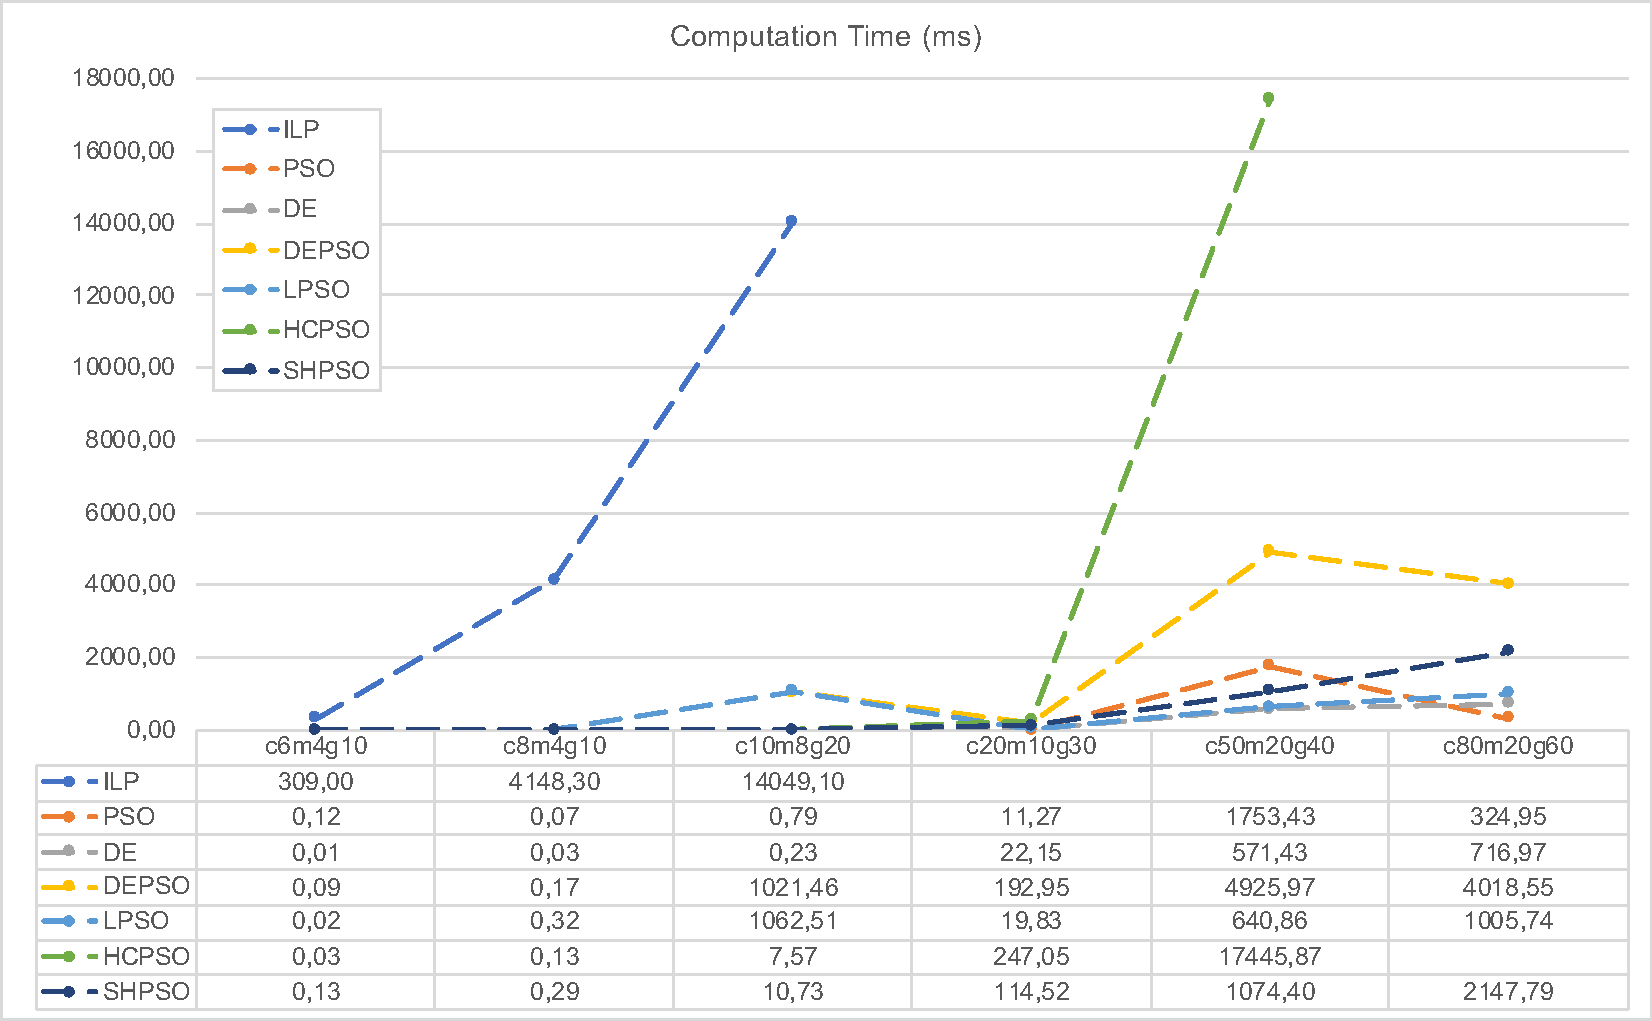
\includegraphics[width=1\linewidth]{img/time_summary.pdf}
\caption{Computation Time of the Various Algorithms for Solving Different Instances of the Software Allocation Problem.}
\label{fig_allocationtime_ilp_metaheuristic}\vspace{-0.4cm}
\end{figure}
%\begin{adjustbox}{angle=90}
\small
% Please add the following required packages to your document preamble:
% \usepackage{booktabs}

\begin{tabular}{@{}llllllllll@{}}
\toprule
Application & method & Fitness &  &  &  & power &  &  &  \\ \midrule
 &  & min & max & avg & std & min & max & avg & std \\
c6, m4,g10 & ILP & 2.28E+02 & 2.28E+02 & 2.28E+02 & 0.00E+00 & 1.58E+02 & 1.58E+02 & 1.58E+02 & 3.00E-14 \\
 & PSO & 2.28E+02 & 2.35E+02 & 2.29E+02 & 2.38E+00 & 1.58E+02 & 1.65E+02 & 1.59E+02 & 2.38E+00 \\
 & DE & 2.28E+02 & 2.28E+02 & 2.28E+02 & 3.00E-14 & 1.58E+02 & 1.58E+02 & 1.58E+02 & 3.00E-14 \\
 & DEPSO & 2.28E+02 & 2.29E+02 & 2.28E+02 & 3.08E-01 & 1.58E+02 & 1.59E+02 & 1.58E+02 & 3.09E-01 \\
 & LPSO & 2.28E+02 & 2.28E+02 & 2.28E+02 & 3.00E-14 & 1.58E+02 & 1.58E+02 & 1.58E+02 & 3.00E-14 \\
 & HCPSO & 2.28E+02 & 2.28E+02 & 2.28E+02 & 3.00E-14 & 1.58E+02 & 1.58E+02 & 1.58E+02 & 3.00E-14 \\
 & SHPSO & 2.28E+02 & 2.28E+02 & 2.28E+02 & 3.00E-14 & 1.58E+02 & 1.58E+02 & 1.58E+02 & 3.00E-14 \\
c8, m6,g20 & ILP & 4.07E+02 & 4.07E+02 & 4.07E+02 & 5.99E-14 & 3.17E+02 & 3.17E+02 & 3.17E+02 & 0.00E+00 \\
 & PSO & 4.07E+02 & 4.44E+02 & 4.15E+02 & 1.24E+01 & 3.17E+02 & 3.44E+02 & 3.23E+02 & 8.70E+00 \\
 & DE & 4.07E+02 & 4.09E+02 & 4.07E+02 & 1.05E+00 & 3.17E+02 & 3.19E+02 & 3.17E+02 & 1.05E+00 \\
 & DEPSO & 4.07E+02 & 4.35E+02 & 4.10E+02 & 8.80E+00 & 3.17E+02 & 3.35E+02 & 3.19E+02 & 5.64E+00 \\
 & LPSO & 4.07E+02 & 4.08E+02 & 4.07E+02 & 5.33E-01 & 3.17E+02 & 3.18E+02 & 3.17E+02 & 5.33E-01 \\
 & HCPSO & 4.07E+02 & 4.07E+02 & 4.07E+02 & 5.99E-14 & 3.17E+02 & 3.17E+02 & 3.17E+02 & 0.00E+00 \\
 & SHPSO & 4.07E+02 & 4.07E+02 & 4.07E+02 & 5.99E-14 & 3.17E+02 & 3.17E+02 & 3.17E+02 & 0.00E+00 \\
c10, m8,g20 & ILP & 4.42E+02 & 4.42E+02 & 4.42E+02 & 5.99E-14 & 2.82E+02 & 2.82E+02 & 2.82E+02 & 5.99E-14 \\
 & PSO & 4.42E+02 & 4.74E+02 & 4.49E+02 & 1.26E+01 & 2.82E+02 & 3.44E+02 & 2.95E+02 & 2.53E+01 \\
 & DE & 4.42E+02 & 4.97E+02 & 4.52E+02 & 1.77E+01 & 2.82E+02 & 3.67E+02 & 3.05E+02 & 3.58E+01 \\
 & DEPSO & 4.42E+02 & 4.43E+02 & 4.42E+02 & 1.90E-01 & 2.82E+02 & 2.83E+02 & 2.82E+02 & 1.90E-01 \\
 & LPSO & 4.42E+02 & 4.43E+02 & 4.42E+02 & 1.70E-01 & 2.82E+02 & 2.83E+02 & 2.82E+02 & 1.70E-01 \\
 & HCPSO & 4.42E+02 & 4.43E+02 & 4.43E+02 & 2.09E-01 & 2.82E+02 & 2.83E+02 & 2.83E+02 & 2.09E-01 \\
 & SHPSO & 4.42E+02 & 4.43E+02 & 4.42E+02 & 1.92E-01 & 2.82E+02 & 2.83E+02 & 2.82E+02 & 1.92E-01 \\
c20, m10,g30 & ILP & NA & NA & NA & NA & NA & NA & NA & NA \\
 & PSO & 5.69E+04 & 8.72E+04 & 6.46E+04 & 9.54E+03 & 1.69E+03 & 2.44E+03 & 2.08E+03 & 2.52E+02 \\
 & DE & 4.71E+04 & 6.22E+04 & 5.37E+04 & 4.13E+03 & 2.06E+03 & 2.30E+03 & 2.15E+03 & 6.56E+01 \\
 & DEPSO & 3.71E+04 & 5.22E+04 & 4.41E+04 & 4.24E+03 & 1.93E+03 & 2.17E+03 & 2.03E+03 & 8.84E+01 \\
 & LPSO & 4.73E+04 & 6.73E+04 & 5.86E+04 & 6.62E+03 & 1.66E+03 & 2.32E+03 & 2.10E+03 & 1.90E+02 \\
 & HCPSO & 4.19E+04 & 4.71E+04 & 4.25E+04 & 1.64E+03 & 1.82E+03 & 2.13E+03 & 1.93E+03 & 1.27E+02 \\
 & SHPSO & 3.73E+04 & 4.70E+04 & 4.26E+04 & 2.77E+03 & 1.93E+03 & 2.28E+03 & 2.04E+03 & 1.14E+02 \\ \bottomrule
\end{tabular}
\end{adjustbox}

\begin{adjustbox}{angle=90}
\small
% Please add the following required packages to your document preamble:
% \usepackage{booktabs}

\begin{tabular}{@{}llllllllll@{}}
\toprule
Application & method & Fitness &  &  &  & power &  &  &  \\ \midrule
 &  & min & max & avg & std & min & max & avg & std \\
c50, m20,g60 & ILP & NA & NA & NA & NA & NA & NA & NA & NA \\
 & PSO & 1.23E+06 & 1.36E+06 & 1.30E+06 & 3.86E+04 & 7.70E+03 & 9.21E+03 & 8.67E+03 & 4.78E+02 \\
 & DE & 1.39E+06 & 1.50E+06 & 1.46E+06 & 3.46E+04 & 8.67E+03 & 1.01E+04 & 9.50E+03 & 5.55E+02 \\
 & DEPSO & 1.33E+06 & 1.45E+06 & 1.38E+06 & 3.26E+04 & 8.46E+03 & 1.05E+04 & 9.43E+03 & 7.21E+02 \\
 & LPSO & 1.38E+06 & 1.48E+06 & 1.43E+06 & 3.20E+04 & 7.94E+03 & 9.90E+03 & 8.81E+03 & 6.19E+02 \\
 & HCPSO & 1.23E+06 & 1.41E+06 & 1.28E+06 & 6.53E+04 & 5.90E+03 & 7.73E+03 & 7.11E+03 & 6.41E+02 \\
 & SHPSO & 1.23E+06 & 1.41E+06 & 1.34E+06 & 9.81E+04 & 5.90E+03 & 7.32E+03 & 6.61E+03 & 1.00E+03 \\
c80, m20,g60 & ILP & NA & NA & NA & NA & NA & NA & NA & NA \\
 & PSO & 2.65E+06 & 2.74E+06 & 2.69E+06 & 4.60E+04 & 7.63E+03 & 1.06E+04 & 9.27E+03 & 1.52E+03 \\
 & DE & 2.71E+06 & 2.76E+06 & 2.74E+06 & 2.38E+04 & 8.55E+03 & 1.20E+04 & 1.07E+04 & 1.89E+03 \\
 & DEPSO & 2.55E+06 & 2.63E+06 & 2.60E+06 & 4.69E+04 & 1.01E+04 & 1.23E+04 & 1.09E+04 & 1.18E+03 \\
 & LPSO & 2.61E+06 & 2.68E+06 & 2.65E+06 & 3.58E+04 & 1.07E+04 & 1.12E+04 & 1.10E+04 & 2.50E+02 \\
 & HCPSO & NA & NA & NA & NA & NA & NA & NA & NA \\
 & SHPSO & 2.40E+06 & 2.57E+06 & 2.47E+06 & 8.94E+04 & 5.25E+03 & 7.34E+03 & 6.52E+03 & 1.12E+03 \\ \bottomrule
\end{tabular}
\end{adjustbox}
% Please add the following required packages to your document preamble:
% \usepackage{booktabs}
\begin{table}[]
\small
\begin{tabular}{@{}lllllll@{}}
\toprule
Sample & Algorithm & \multicolumn{2}{c}{Fitness} & \multicolumn{2}{c}{Time (ms)} & Quality \\ \midrule
 &  & Mean & SD & Mean & SD &  \\ \midrule
\pb{6}{10}{4} 
 & \textbf{ILP} & 227.88 & 0 & 309 & 57.74 & 100.00  \\
 & PSO & 229.11 & 2.38 & 0.12 & 0.34 & 99.46  \\
 & DE & 227.88 & 0 & 0.01 & 0 & 100.00  \\
 & DEPSO & 228.07 & 0.31 & 0.09 & 0.01 & 99.92  \\
 & LPSO & 227.88 & 0 & 0.02 & 0.02 & 100.00  \\
 & HCPSO & 227.88 & 0 & 0.03 & 0 & 100.00  \\
 & SHPSO & 227.88 & 0 & 0.13 & 0.03 & 100.00  \\
\pb{8}{20}{6} 
 & \textbf{ILP} & 406.6 & 0 & 4148.3 & 95.77 & 100.00  \\
 & PSO & 415.15 & 12.4 & 0.07 & 0.15 & 97.94  \\
 & DE & 407.42 & 1.05 & 0.03 & 0.02 & 99.80  \\
 & DEPSO & 409.65 & 8.8 & 0.17 & 0.01 & 99.26  \\
 & LPSO & 407.18 & 0.53 & 0.32 & 0.73 & 99.86  \\
 & HCPSO & 406.6 & 0 & 0.13 & 0.06 & 100.00  \\
 & SHPSO & 406.6 & 0 & 0.29 & 0.14 & 100.00  \\
\pb{10}{20}{8} 
 & \textbf{ILP} 
 & 442.37 & 0 & 14049.1 & 150.84 & 100.00  \\
 & PSO & 448.79 & 12.61 & 0.79 & 1.37 & 98.57  \\
 & DE & 451.55 & 17.72 & 0.23 & 0.41 & 97.97  \\
 & DEPSO & 442.44 & 0.19 & 1021.46 & 2263.76 & 99.98  \\
 & LPSO & 442.49 & 0.17 & 1062.51 & 2338.73 & 99.97  \\
 & HCPSO & 442.67 & 0.21 & 7.57 & 22.68 & 99.93  \\
 & SHPSO & 442.46 & 0.19 & 10.73 & 61.31 & 99.98  \\
\pb{20}{30}{10} 
 & ILP & NA & NA & NA & NA & NA \\
 & PSO & 64595.28 & 9544.82 & 11.27 & 9.73 & 65.74  \\
 & DE & 53655.73 & 4134.84 & 22.15 & 7.95 & 79.14  \\
 & DEPSO & 44055.97 & 4237.81 & 192.95 & 230.83 & 96.38  \\
 & LPSO & 58603.42 & 6617.49 & 19.83 & 6.98 & 72.46  \\
 & \textbf{HCPSO} & 42462.38 & 1643.71 & 247.05 & 104.36 & 100.00  \\
 & SHPSO & 42558.2 & 2770.52 & 114.52 & 102.41 & 99.77  \\
\pb{50}{60}{20} 
 & ILP & NA & NA & NA & NA & NA \\
 & PSO & 1298680.85 & 38557.68 & 1753.43 & 776.16 & 98.26  \\
 & DE & 1460553.62 & 34599.66 & 571.43 & 248.46 & 87.37  \\
 & DEPSO & 1384474.66 & 32550.41 & 4925.97 & 4809.57 & 92.17  \\
 & LPSO & 1430847.88 & 32045.32 & 640.86 & 320.33 & 89.18  \\
 & \textbf{HCPSO}
 & 1276036.05 & 65320.02 & 17445.87 & 15796.87 & 100.00  \\
 & SHPSO & 1336679.78 & 98051.36 & 1074.4 & 339.83 & 95.46  \\
\pb{80}{60}{20} 
 & ILP & NA & NA & NA & NA & NA \\
 & PSO & 2692638.14 & 46015.42 & 324.95 & 103.66 & 91.60  \\
 & DE & 2737416.39 & 23780.06 & 716.97 & 207.19 & 90.10  \\
 & DEPSO & 2604249.6 & 46945.89 & 4018.55 & 12.37 & 94.71  \\
 & LPSO & 2650992.23 & 35813.35 & 1005.74 & 375.25 & 93.04  \\
 & HCPSO & NA & NA & NA & NA & NA \\
 & \textbf{ } & 2466535.41 & 89380.36 & 2147.79 & 357.58 & 100.00  \\ \bottomrule
\end{tabular}
\caption{Fitness and Allocation Time of the ILP and the Metaheuristic Techniques, for the Increasing Sizes of the Software Allocation Problem.}
\label{tbl_fitness_allocationtime_ilp_plus_metaheuristic}
\end{table}

\section{Discussion}
